\section{Field Trialling AtomicOrchid}\label{sec:evaluation}
\noindent We ran three sessions of AtomicOrchid with participants recruited from the local university to trial mixed-initiative coordination in a disaster response scenario. The following sections describe the participants, procedure, session configuration and methods used to collect and analyse quantitative and qualitative data.

\subsection{Participants and Procedure}
%\noindent We do not attempt to run tens or hundreds of trials to generate statistically significant results. Rather, we focus on running enough trials to gain an insight into how participants perceive and interact with our planning agent. This approach is advocated in  \cite[p. 1663]{Brown:2011:WCO:1978942.1979185}, in which participants in field trials are experts on their own activity.  These experts attempt to predict what might happen with a particular technology, to develop insights based on their use of it.  In particular,  \cite{Brown:2011:WCO:1978942.1979185} point to the fact that running multiple trials (in an attempt to obtain statistical significant results)  has no relationship to  insightfulness.  Crucially, they suggest that  participants can be seen as investigators themselves in the  trial, with a move to acknowledging that it is through  participants' own insights that the power of the trials can be focused.
%


%\noindent As argued by \cite[p. 1663]{Brown:2011:WCO:1978942.1979185}, participants in field trials are used as experts on their own activity, attempting to predict what might happen with  a particular technology, to develop insight based on their  use.  In particular, they point to the fact that running multiple trials (in an attempt to obtain statistical significant results)  has no relationship to  insightfulness.  Crucially, they suggest that  participants can be seen as investigators themselves in the  trial, with a move to acknowledging that it is through  participants� own insights that the power of the trials can be focused. Hence, in line with this argument, we do not attempt to run tens or hundreds of trials to generate statistically significant results. Rather, we focus on running enough trials to gain an insight into how participants perceive and interact with our planning agent.
%

\noindent We do not attempt to run tens or hundreds of trials to generate statistically significant results. Instead, our approach to field trials is strongly influenced by \cite[p. 1663]{Brown:2011} who state that ``participants in field trials are used as experts on their own activity, attempting to predict what might happen with  a particular technology, to develop insight based on their  use".  In particular, they point to the fact that running multiple trials (in an attempt to obtain statistically significant results)  has no relationship to  insightfulness.  Crucially, they suggest that  participants can be seen as investigators themselves in the  trial. Hence, in line with this argument, we do not attempt to run tens or hundreds of trials on many different scenarios to generate statistically significant results. Rather, we focus on running enough trials to gain an insight into how participants \emph{perceive} and \emph{interact} with our planning agent.

Hence, a total of 24 participants (17 males and 7 females) were recruited through posters and emails, and reimbursed with \pounds 15  for 1.5-2 hours of study. The majority were students. The procedure consisted of 30 minutes of game play, and about 1 hour in total of pre-game briefing, consent forms,  a short training session, and a post-game group discussion. The participants were told that their goal was to save as many targets as possible out of 20. This was enough to motivate them (as we saw in the runs) to actively engage with the game mechanics in order to collect as many targets as possible.

%Upon arrival in the HQ (set up in a meeting room at the local university), participants were briefed and asked to consent to participate. They were presented with a demographic questionnaire to record gender, occupation, experience of using smartphones and level of map navigation skills.

At the end of the briefing, in which mission objectives and rules were outlined, FR types were randomly assigned to all participants (fire-fighter, medic, transporter, soldier). The HQ was staffed by a different member of the research team in each session in order to mimic an experienced $H$, while avoiding the same person running the HQ every time.  Moreover, FRs were provided with a smartphone and $H$ with a laptop. The team was given 5 minutes to discuss a common game strategy. 

FRs were then accompanied to the starting point within the designated game area, about 1 minute walk from headquarters. Once FRs were ready to start, $H$ sent a `game start' message. After 30 minutes of game play the FRs returned to the HQ where a group interview was conducted, before participants were debriefed and dismissed.

\subsection{Game Sessions}
\noindent We ran one session without $PA$, and two sessions with $PA$ to be able to compare team performance in the two versions. Each session involved \emph{different} sets of FRs (8 each). Thus,  players were unique to a session to avoid learning effects between sessions. While we cannot rule out learning effects \textit{within} sessions, we accept this as an integral part of working with humans in the real world. 

We also ran a pilot study for each condition to fine tune game configuration. The 8 FRs in each session were randomly allocated a role so that the whole team had two of each of the four types of FRs. The terrain of the 400x400 metre  game area includes grassland, a lake, buildings, roads,  footpaths and lawns. There were two  drop-off zones and 16 targets in each session. There were four targets for each of the four target types. The target locations, pattern of cloud movement and expansion were kept constant for all game sessions. The pilot study showed that this was a challenging, yet not too overwhelming configuration of game area size, and number of targets to collect in a 30 min game session. 

\subsection{Data Collection and Analysis}
\noindent We collected more than 20 hours of video of participants at the HQ, and participants on the ground (using multiple cameras to follow multiple teams at the same time). Video recordings of field action were catalogued to identify sequences (episodes) of interest through identification of key decision points in teaming and task allocation. Interesting distinct units of interaction were transcribed and triangulated with log files of relevant game activity for qualitative interaction analysis, presented in detail elsewhere \cite{Jiang2014}. For the purposes of the analysis presented here, we analysed the video data to classify how the agent task allocations were handled by humans. 

In addition, we developed a log file replay tool to triangulate video recordings of game action with the timestamped system logs that contain a complete record of the game play, including FRs' GPS location, their health status and radioactive exposure, messages, cloud location, locations of target objects and task status.

%Video recordings of field action were catalogued to identify sequences (episodes) of interest (cf. Heath et al., 2010). Key decision points in teaming and task allocation served to index the episodes. Interesting distinct units of interaction were transcribed and triangulated with log files of relevant game activity for deeper analysis. Due to space constraints we can only  present one fragment in this paper to illustrate how human-agent collaboration typically unfolded (TODO).

In this paper, we present an analysis of both $PA$'s task allocations and the messages sent between FRs and $H$ to support coordination in order to assess how humans interact with each other and with $PA$. In particular, we use speech-act theory \cite{searle:1975} to classify the messages composed by humans. We focus on the most relevant types of acts in this paper (which are also the most frequently used in AtomicOrchid):

\begin{itemize}
\item Assertives: \textit{speech acts that commit a speaker to the truth of the expressed proposition}; these were a common category as they include messages that contain situational information (e.g., You are next to the radiation cloud or the task is North of your current position).
\item Directives: \textit{speech acts that are meant to cause the hearer to take a particular action}; requests, commands and advice, including task and team allocation messages (e.g., X go to task 1, Y go with X).
\end{itemize}

\subsection{Results}
\noindent  The participants were seen to engage engage with the game scenario, showing signs of stress when targets could not be saved, and at times, running to save targets before these were covered by the radioactive cloud. This confirmed that the fun factor of the game helped to incentivise the participants to optimise their task allocation plans. 

Overall, 8 targets were rescued in the non-agent condition (Session A), and respectively 12 targets (Session B) and 11 targets (Session C) were rescued in the agent condition. Teams (re-)formed six times in session A, four times in session B and nine times  in session C. Average player health after the game was much higher (more than double) for the agent-assisted sessions (91 for Session B and 72 for Session C) compared to the non-agent assisted session (40 in Session A) (see table \ref{tab:health}). In fact, one FR `died' in Session A. This suggests that the agent's more conservative approach not to send FRs  into 'harms way' paid off. Moreover, surprisingly this more conservative approach did also not result in fewer  targets saved than with a, perhaps, more risk seeking approach by HQ in Session A. This may  be explained by more timely instructions by the agent, as these were generated automatically after a target had been dropped off.  

$PA$ dynamically re-planned 14 times in session B and 18 times in session C. In most cases, this was triggered when a target was dropped off in the safe zone (24 times) -- as this frees up resources for  $PA$ to recompute an allocation. In the remaining cases, this was triggered by a player declining the agent's task allocation (8 times). 


\begin{table}[ht]\small\centering
 \caption{Health of FRs}\begin{tabular}{c | c | c | c | c}
 & Minimum health &  Maximun health & Average health & Standard deviation \\
 \hline
 Session A & 0 & 95 & 40 & 26.95  \\
  \hline
  Session B & 64 & 100 & 91 & 13.41   \\
  Session C & 41 & 99 & 72 & 24.99   \\
\end{tabular}\label{tab:health}
\end{table}


%\subsubsection{Handling Task Allocations}
In particular, Figure \ref{fig:msgs} shows how FRs handled task allocations in the agent and  non-agent conditions. In the non-agent condition, the HQ commander sent 43 task allocation directives (see Table \ref{tab:assertives} for details of each run) . Of these, the recipient FRs addressed only 15 messages (bringing them up in conversation). Of these 15, FRs chose to ignore the instructions only once. The FRs ignored the instruction because they were engaged in another task and did not want to abandon it. A further 4 $H$ instructions were consistent with a decision to rescue a certain target that had already been agreed locally by the FRs. In the remaining 10 cases,  FRs chose to follow the instructions. Although players were willing to follow $H$'s instructions, they failed to correctly follow the instructions due to confusion and misunderstanding in the communication. In fact, only 2 instances of directives from $H$ led to task completion. The FRs performed 6 rescue operations (tasks) without being instructed by $H$.

\begin{figure}[t]
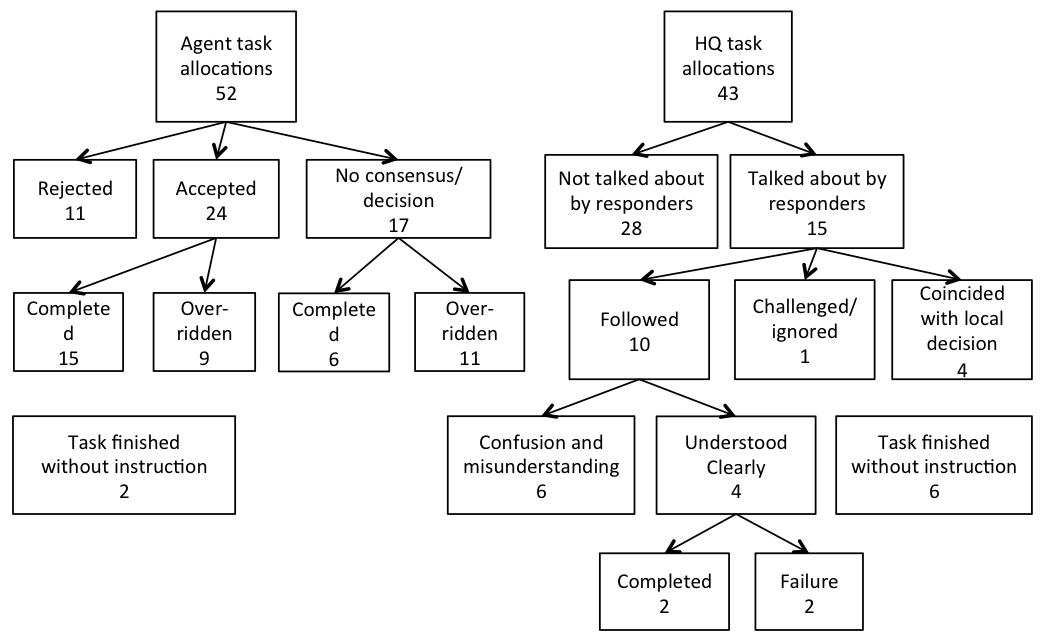
\includegraphics[width=\columnwidth]{message_handling.png}
\vspace{-5mm}
\caption{How task allocations were handled by FRs in the version with agent (left), and without agent (right). The `overridden' box denotes the number of times an `accepted' allocation in the non-agent case was not carried out to its full extent and, instead, another task was chosen by $H$ to be completed.}\label{fig:msgs}
\end{figure}


\begin{table}[ht]\small\centering
 \caption{Message classification.} \label{tab:msgs}
\begin{tabular}{c | c c | c c c c | c}
 & \multicolumn{2}{c|}{no agent} &  \multicolumn{4}{c|}{agent} & Total \\
 \hline
 Speech acts & \multicolumn{2}{c|}{Session A} & \multicolumn{2}{c}{Session B} & \multicolumn{2}{c|}{Session C} & \\
  & HQ & FR & HQ & FR & HQ & FR & \\
  \hline
  Directives & 89 & 0 & 34 & 2 & 34 & 0 & 159 \\
  Assertives & 33 & 6 & 26 & 16 & 24 & 16 & 121 \\
  \hline
  Total & 122 & 6 & 60 & 18 & 58 & 16 & 280 \\
\end{tabular}
\label{tab:assertives}
\end{table}


In contrast, when task allocation was handled by the agent (52 tasks allocated in two trials on average), FRs explicitly accepted 24 tasks,  of which they completed 15  successfully. Although there was either no response or no consensus between the FRs (in 17 tasks allocated), they still completed 6 of these tasks successfully. In total, 20 task allocations were withdrawn by the agent as a result of re-planning. 



%\paragraph{Rejecting task allocations}
In terms of task rejections, FRs rejected $PA$'s task allocation 11 times in the agent version. All of the rejections happened when the task allocation would have \emph{split existing teams}, or instructed FRs to team up with \emph{physically more distant FRs}. In most cases (9 out of 11), they triggered re-planning by rejection and \emph{adjusted the task allocation} to become consistent with the FR's current team. In the other two cases, the FRs rejected  the task allocation one more time before receiving the desired task allocation. For accepted instructions, the average distance between suggested teammates was 12 metres. For rejected instructions, the average was 86 metres.

The results above show that  the simple mechanism to get $PA$ to re-plan (i.e., reject/accept) was more successful (more tasks completed and less confusion) than the open-ended interactions between $H$ and the FRs (that were open to confusion).  Moreover, the fact that many of the rejections were due to the long distance to travel and teammate preference, implies that players chose to do the tasks they \emph{preferred}  rather than those deemed optimal by the agent. This indicates there may be an issue of trust in the agent, but also that it may be easier for a FR  to impose (through a reject) such preferences on an agent (and indirectly to other team members) rather than expressing this to $H$ or directly to teammates. 
% Role of HQ commander
It is also important to note that in the agent-assisted setting, $H$ frequently \emph{monitored} the allocation of tasks  returned by the agent (57 clicks on `show task' in UI FR status widget). Whereas 43 directives out of 68 in the non-agent session were task allocations, only 16 out of 68 were directly related to task allocations in the agent version. Out of these, $H$ directly reinforced the agent's instruction 6 times (e.g., ``SS and LT retrieve 09''), and complemented (i.e., added to or elaborated) $PA$'s task allocation 5 times (e.g., ``DP and SS, as soon as you can head to 20 before the radiation cloud gets there first''). $H$  did `override' $PA$'s instruction in 5 cases (as depicted by the `overridden' box).  

In the agent version, most of $H$'s directives (52 out of 68) and assertives (49 out of 51) focussed on providing situational awareness and  routing the FRs to avoid exposing them to radiation. For example, ``NK and JL approach drop off 6 by navigating via 10 and 09.'', or ``Radiation cloud is at the east of the National College''. 

These quantitative results point to the fact that H used PA as an advisor and in the non-agent case, H had to provide more information to FR on the ground. In fact,  during the debriefing session, the HQ operators in the non-agent case explicitly mentioned being overloaded by the number of variables under consideration when allocating tasks to FRs (e.g., providing situational awareness and allocating tasks) However, when supported by PA, the participants mentioned they trusted the agent to make the right decision and mainly spent time supervising its allocations or even improving the allocation in some cases. For example, in one instance, H explicitly advised FRs to go for a task that PA calculated would be covered by the radiation cloud before they could get there.  However, PA's estimates of FRs' running speed was obviously wrong in this case and the FRs were able to rescue the target. 


%\subsubsection{Summary and Guidelines}\label{sec:summary}
In summary, these results suggest three key observations with regard to  human-agent coordination in the trial: 
\begin{enumerate}
\item FRs performed better (rescued more targets)  and maintained higher health levels when supported by the agent.  These results echo those obtained under simulation (see Appendix \ref{sec:appendix2}) and  may reflect the better forward-planning capability of the planning agent compared to human FRs. 
 
\item Rejecting tasks was relatively frequently employed to trigger re-planning to obtain new task allocations aligned with FR preferences.  In each case, the planning agent was able to adapt to provide an alternative  that was acceptable to the FRs. Without this facility we believe the FRs would have chosen to ignore the plan. Task rejection seemed to be linked to changes to established teams, especially when members were relatively distant. Consequently, these kinds of allocations may need particularly support (e.g., explanation) or might be less preferentially selected by $PA$.

\item When task allocation was handled by $PA$, $H$ could focus on providing vital situational awareness to safely route first FRs around danger zones: thus demonstrating effective division of labour and complementary collaboration between humans and agents.
\end{enumerate}

Given the above observation we argue that a planning agent for team formation should not only model the uncertainty in player behaviours and in the environment, but that interactional challenges also need to be addressed  if such a technology is to be accepted in practice.  In the next section we elaborate on how our study results lead to new design guidelines for Human-Agent Collectives.

%\todo{--Gopal? Think this one's for you? (JF) -- the conclusions call for flexible autonomy, and this is somewhat supported by the algorithm and results. There are a few important limitations that the authors should discuss. For example, it is possible for responders to reject enough tasks tha the mission becomes infeasible. How would such a problem be addressed? The solution to such problems is beyond the scpoe of the paper but the relevant limitations of the algorithms are not.
%}

